\begin{figure}[H]
\caption{Kappa Architecture}
\centering
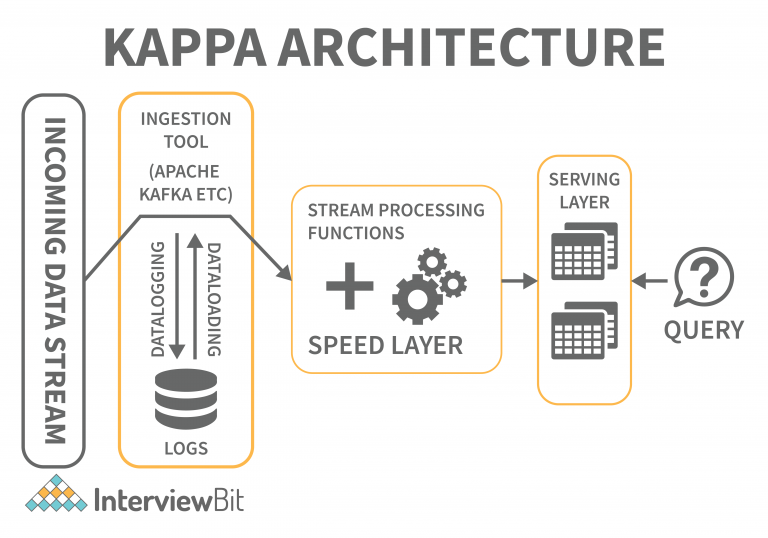
\includegraphics[width=1\linewidth]{images/Kappa-Architecture-768x538.png}
\small
\textit{Note.} The image depicts the Kappa Architecture, which is a data processing framework designed for handling real-time data streams. \textbf{Incoming Data Stream} — The starting point of the data flow; \textbf{Ingestion Tool} — Utilizes technologies like Apache Kafka for data intake; \textbf{Stream Processing Functions} — Core data processing layer; \textbf{Speed Layer} — Handles real-time data processing; \textbf{Serving Layer} — Presents processed data for querying; \textbf{Query Interface} — Allows users to interact with the processed data;
\textit{Creator.} (\cite{interviewBit})\footnote[39]{\fullcite{interviewBit}}
\end{figure}